\documentclass[11pt]{article}
\usepackage{geometry,marginnote} % Pour passer au format A4
\geometry{hmargin=1cm, vmargin=1cm} % 

% Page et encodage
\usepackage[T1]{fontenc} % Use 8-bit encoding that has 256 glyphs
\usepackage[english,french]{babel} % Français et anglais
\usepackage[utf8]{inputenc} 

\usepackage{lmodern,numprint}
\setlength\parindent{0pt}

% Graphiques
\usepackage{graphicx,float,grffile,units}
\usepackage{tikz,pst-eucl,pst-plot,pstricks,pst-node,pstricks-add,pst-fun,pgfplots} 

% Maths et divers
\usepackage{amsmath,amsfonts,amssymb,amsthm,verbatim}
\usepackage{multicol,enumitem,url,eurosym,gensymb,tabularx}

\DeclareUnicodeCharacter{20AC}{\euro}



% Sections
\usepackage{sectsty} % Allows customizing section commands
\allsectionsfont{\centering \normalfont\scshape}

% Tête et pied de page
\usepackage{fancyhdr} \pagestyle{fancyplain} \fancyhead{} \fancyfoot{}

\renewcommand{\headrulewidth}{0pt} % Remove header underlines
\renewcommand{\footrulewidth}{0pt} % Remove footer underlines

\newcommand{\horrule}[1]{\rule{\linewidth}{#1}} % Create horizontal rule command with 1 argument of height

\newcommand{\Pointilles}[1][3]{%
  \multido{}{#1}{\makebox[\linewidth]{\dotfill}\\[\parskip]
}}

\newtheorem{Definition}{Définition}

\usepackage{siunitx}
\sisetup{
    detect-all,
    output-decimal-marker={,},
    group-minimum-digits = 3,
    group-separator={~},
    number-unit-separator={~},
    inter-unit-product={~}
}

\setlength{\columnseprule}{1pt}

\begin{document}

\textbf{Nom, Prénom :} \hspace{8cm} \textbf{Classe :} \hspace{3cm} \textbf{Date :}\\

\vspace{-0.5cm} \begin{center}
  \textit{La valeur morale ne peut pas être remplacée par la valeur intelligence et j'ajouterai : Dieu merci !}  - \textbf{Albert Einstein}
\end{center}

\subsection*{Consignes}

\begin{itemize}[label={$\bullet$}]
  \item Il faut dessiner une montre à aiguilles.
  \item Elle doit indiquer l'heure de 14h 50min et 30s.
\end{itemize}

\subsection*{Conseils pour les heures}

\begin{itemize}[label={$\bullet$}]
  \item Le cadran d'une montre est partagé en 12h. Chaque heure est représentée par un index :  un rond, un trait, ...
  \item Les heures sont marquées de 1 à 12.
  \item La petite aiguille indique les heures. 
  \item Comme il est presque 15h. L'aiguille des heures est proche de \dotfill
\end{itemize}

\subsection*{Conseils pour les minutes}

\begin{itemize}[label={$\bullet$}]
  \item La grande aiguille indique les minutes. 
  \item Comme il est presque 14h50. L'aiguille des minutes est sur \dotfill
  \item Un cercle sur le cadran représentant les minutes peut être présent sur certains modèles. 
  \item Un cercle à l'extérieur du cadran peut être présent sur des montres de plongée. On parle de lunette.
\end{itemize}

\subsection*{Conseils pour les secondes}

\begin{itemize}[label={$\bullet$}]
  \item L'aiguille fine qui indique les secondes s'appelle la trotteuse.
  \item L'aiguille des secondes peut ne pas être au même endroit que l'aiguille des heures sur certains modèles. 
\end{itemize}

\subsection*{Remarques}

\begin{itemize}[label={$\bullet$}]
  \item Le dessin doit être "beau" et "colorié".
  \item Le dessin sera plus réussi si la montre a un bracelet.
  \item La marque peut ne pas exister.
  \item Il est conseillé de faire le cadran avec le compas.
\end{itemize}


Quelques photos de montres pour vous aidez : 

\begin{multicols}{4}

\begin{figure}[H]
  \centering
  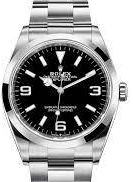
\includegraphics[width=\linewidth]{6x8-temps/rolex.jpeg}
\end{figure}

\begin{figure}[H]
  \centering
  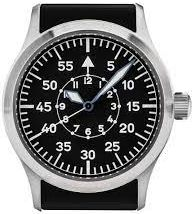
\includegraphics[width=\linewidth]{6x8-temps/stowa.jpeg}
\end{figure}

\begin{figure}[H]
  \centering
  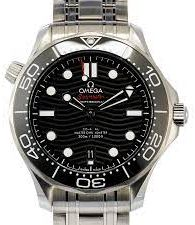
\includegraphics[width=\linewidth]{6x8-temps/omega.jpeg}
\end{figure}

\begin{figure}[H]
  \centering
  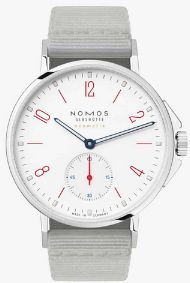
\includegraphics[width=\linewidth]{6x8-temps/nomos.jpeg}
\end{figure}

\end{multicols}

\end{document}